\chapter{Lecture}\label{part3:lec32} %% 32
\markboth{\thechapter. Lecture}{\thechapter. Lecture}

We\pageoriginale shall study a few more properties of Dedekind
sums. We had the reciprocity law
$$
s(h, k)+ s(k, h)=- \frac{1}{4} + \frac{1}{12} \left( \frac{h}{k} +
\frac{k}{h} + \frac{1}{hk}\right).
$$

From this we deduced as a consequence
\begin{equation*}
  12 hk ~s(h, k) \equiv h^2+1 \pmod{k} \tag{*}\label{part3:lec32:eq*}
\end{equation*}

Now when do the Dedekind sums vanish? Let us write $s(h, k)$ in the
more flexible form:
$$
s(h, k)= \sum_{\mu \mod k} \left(\left( \frac{\mu}{k}\right)\right)
\left(\left( \frac{\mu h}{k}\right) \right)
$$

Let $h h^* \equiv 1 \pmod{k}$. Since $(h^*, k)=1$, $h^* \mu$ runs
through a full residue system modulo $k$, and so
\begin{align*}
  s(h, k) & = \sum_{\mu \mod k} \left(\left( \frac{\mu
    h^*}{k}\right)\right)\left(\left( \frac{\mu
    hh^*}{k}\right)\right)\\
  & = \sum_{\mu \mod k} \left(\left( \frac{\mu}{k}\right)\right)
  \left(\left( \frac{\mu h^*}{k}\right)\right)\\
  & = s(h^*, k)
\end{align*}

This is of some significance. We came to $s$ from the substitution
$\left(\begin{smallmatrix} a & b\\ c & d\end{smallmatrix}\right)$ and since
  $ad\equiv 1 \pmod{c}$, $s(d, c)= s(a, c)$. $hh' \equiv -1 \pmod{k}$,
  and 
\begin{align*}
  s(h, k)& = \sum_{\mu \mod k} \left(\left(
  \frac{\mu}{k}\right)\right) \left(\left( \frac{\mu
    h}{k}\right)\right) \\
  & = \sum_{\mu \mod k} \left(\left( \frac{h'\mu}{k}\right)\right)
  \left(\left( \frac{\mu hh'}{k}\right)\right) \\
  & = \sum_{\mu \mod k} \left(\left( -\frac{\mu}{k}\right)\right)
  \left(\left( \frac{h'\mu}{k}\right)\right)\\
  & = -s (h', k)
\end{align*}

When\pageoriginale $h= h'$ i.e., $h^2\equiv - \pmod{k}$ (cg. $2^2 \equiv -
\pmod{5}$)
$$
\displaylines{s(h, k)=- s(h, k)\cr
\text{or} \hfill s(h, k)=0 \qquad if \qquad h^2 \equiv -1
\pmod{k}\hfill  }
$$
(in particular if $h^2 + 1 =k$. I have a conjecture that $s(h, k)\geq
0$ if $h^2 < k$). In fact we can say more. We have the 

\begin{theorem*}
  $12~ s(h, k)$ is en integer only for $h^2 \equiv - 1 (\pmod{k})$ and
  is then equal to zero.
\end{theorem*}

For assume that $12 s(h, k)=$ integer; this implies, because of
(\ref{part3:lec32:eq*}),
that $0\equiv h^2 +1 \pmod{k}$

In such cases, therefore, we can make a direct statement about the
value of $s(h, k)$ without going through the rigmarole of the
Euclidean algorithm. Thus $s(2, 5)=0$, $s(5, 26)=0$.

In a recent issue of the Duke Mathematical Journal (1954), I gave a
generalisation of the reciprocity formula for Dedekind sums. It takes
into account three summands. The formula is very elegant and throws
some light on the reciprocity relation itself. We quote it without
proof. 

\begin{theorem*}
  If $a$, $b$, $c$ are pairwise coprime and $aa^* \equiv 1 \pmod{bc}$, $bb^*
  \equiv 1 \pmod{ca}$, $cc^* \equiv 1 \pmod{ab}$, then 
  \begin{align*}
  T & \equiv s(bc^*, a) + s(ca^*, b)+ s(ab^*, c)\\ 
  & =- \frac{1}{4} +
  \frac{1}{2} \left( \frac{a}{bc} + \frac{b}{ca} + \frac{c}{ab}\right)
  \end{align*}
\end{theorem*}\pageoriginale

The proof is by an algebraic method due to R\'edel. The formula is
very gratifying as a generalisation of the reciprocity formula is
which latter there is some non-homogeneity. Put $c=1$; then $c^*=1$,
and $s(ab^*, c)=0$; so we get the reciprocity formula. The right side
above is $\frac{1}{12 ~abc} - 3 abc +a^2 +b^2 +c^2$. Hence $T=0$ if
and only if $a^2+b^2+c^2=3abc$. This combination of three integers
plays some role the theory of quadratic forms; it is called a Markoff
triple. It has reappeared in literature in connection with the
geometry of numbers. It has to do with the existence if certain
quadratic forms with minimum values close to zero for integers. 1, 1,
2 is a Markoff triple. If we keep two of them fixed, for the third we
get a quadratic equation of which one root we know to be rational. So
the other root is rational too. For instance if $a, b =1$ are fixed,
we have $c^2-3c +2=0$ or $(c-1)(c-2)=0$; -- the triples pre 1, 1, 1
and 1,1,2. If we take the triple $a$, 1, 2, then $a^2 + 5 =6a$ or
$a=1,5$; we have the triples $b$, 1, 2; 1, 1, 2. $T=0$ only if $a$,
$b$, $c$ being to a Markoff triple. For such a triple, 
$$
\displaylines{b^2 + c^2 \equiv 0 \pmod{a}, c^2 +a^2 \equiv 0\pmod{b},
  a^2 + b^2\equiv 0 \pmod{c}\cr
  \text{So} \hfill b^2 \equiv - c^2 \pmod{a}, ~\text{or}~  (c^* b)^2
  \equiv -1 \pmod{a}, etc. \hfill }
$$ 

Then $s(bc^*, a)=0$, and each summand in $T$ is zero.

Dedekind sums have something to do with Farey fractions. Let us
suppose that $\left| \begin{smallmatrix} a & b\\ c&
  d \end{smallmatrix}\right| =1, c, d>0$.
$$
\displaylines{s(c, d)+s(d, c)= - \frac{1}{4} + \frac{1}{12}
  \left(\frac{c}{d} + \frac{d}{c} + \frac{1}{cd} \right)\cr
  cb \equiv -1 \pmod{d} ~\text{and}~ ad \equiv 1 \pmod{c}\cr
  \text{so}\hfill s(c, d) =- s(-b, d)~\text{and}~ s(d, c) = s(a,
  c). \hfill \cr
  \text{So}\hfill s(a, c) - s(b, d) =-4 + \frac{1}{12}
  \left(\frac{c}{d} + \frac{d}{c} + \frac{1}{cd} \right)\hfill }
$$

Now\pageoriginale if $\frac{h_1}{k_1}$, $\frac{h_2}{k_2}$ the adjacent Farey
Fractions, then $\left| \begin{smallmatrix} h_1 & h_2\\ k_1 & k_2
\end{smallmatrix}\right|=-1$

so
$$
s(h_1, k_1)-s(h_2, k_2) = \frac{1}{4} - \frac{1}{12}
\left(\frac{k_1}{k_2} + \frac{k_2}{k_1} + \frac{1}{k_1 k_2} \right) 
$$

Write the left side as $s\left(\frac{h_1}{k_1} \right)-
s\left(\frac{h_2}{k_2} \right)$. 

Suppose $\frac{h_2}{k_2}$ is fixed. Let us look at all possible
adjacent fractions  $\frac{h_1}{k_1}$. They are
obtainable by forming mediants; replace $\frac{h_1}{k_1}$ successively
by $\frac{h_1+ \lambda h_2}{k_1 + \lambda k_2}$. Make $k_1$ larger and
larger. Then $\frac{k_2}{k_1}$ and $\frac{1}{k_1 k_2} \to 0$. So
$\frac{k_1}{k_2}\to \infty$. Thus $s\left(\frac{h_1}{k_1}\right) - s
\left(\frac{h_2}{k_2} \right)$ goes unboundedly by $ - \infty$, and so
$s\left( \frac{h_1}{k_1}\right)\to - \infty$. Therefore only on the
left side of $\frac{h_2}{k_2}$ can we get a sequence of rational
fractions for which the Dedekind sums tend to $- \infty$.

We now give another proof of the reciprocity law, by the method of
finite Fourier series, $\left( \left(\frac{\mu}{k} \right)\right)$ is
a number- theoretic periodic function. It has a finite Fourier
expansion:
$$
\left( \left(\frac{\mu}{k} \right)\right)= \sum^k_{j=1} c_j e^{2 \pi i
j \frac{\mu}{k}}
$$   

In fact this is always solvable for $c_1, c_2, \ldots, c_k$. For
writing down\pageoriginale $\mu = 1, 2, 3, \ldots , k$ in succession,
we have a system of $k$ linear equations whose determinant is a
Vandermonde determinant which is non-zero since the roots of unity are
different. We have
\begin{alignat*}{4}
  && \sum^k_{\mu=1} \left( \left(\frac{\mu}{k} \right)\right) e^{-2 \pi
  i \mu \frac{\ell}{k}}&  =\sum^k_{j=1} c_j \sum^k_{\mu=1} e^{2 \pi i
    \mu \frac{(j-\ell)}{k}}\\
  &&& =kc_l,\\
  \text{i.e.,}&\hspace{1cm}& c_l & = \frac{1}{k} \sum^k_{\mu=1} \left(
  \left(\frac{\mu}{k} \right)\right) e^{-2 \pi i \mu \frac{\ell}{k}}\hspace{3cm}
\end{alignat*}

This was done by Eisenstein, We can also write
\begin{align*}
  c_l & = \frac{1}{k} \sum^{k-1}_{\mu=1} \left( \frac{\mu}{k} -
  \frac{1}{2}\right) e^{-2\pi i \mu \frac{l}{k}}\\
  & = \frac{1}{k^2} \sum^{k-1}_{\mu=1} \mu e^{-2 \pi i \mu
    \frac{l}{k}} - 
  \begin{cases}
    \frac{k-1}{2k}, & \text{if}~ k\mid l;\\
    \frac{1}{2k}, & \text{if} ~ k \nmid l.
  \end{cases}
\end{align*}

So if $k \mid l$, then 
$$
c_\ell = \frac{1}{k^2} \frac{k(k-1)}{2} - \frac{k-1}{2k} =0.
$$

In particular 
$$
c_k =0.
$$

If $k \nmid l$, then writing 
\begin{align*}
  S & = \sum^{k-1}_{\mu=1} \mu e^{-2 \pi i \mu
    \frac{\ell}{k}},\\
  S e^{-2 \pi i \frac{\ell}{k}} & = \sum^{k-1}_{\mu=1} \mu e^{-2 \pi i
    \frac{\mu+1}{k} \ell}\\
  & = \sum^k_{\nu=2} (\nu-1) e^{- 2 \pi i \nu \frac{\ell}{k}}\\
  & = S- e^{-2 \pi i \frac{l}{k}} + k - \sum^k_{\nu=1} e^{-2 \pi i
    \nu \frac{l}{k}} + e^{-2 \pi i \frac{l}{k}}
\end{align*}

So\pageoriginale 
$$
S= \frac{k}{e^{- 2 \pi i \ell/k}-1}
$$

Hence, if $k \nmid l$, then
\begin{align*}
  c_\ell & = \frac{-1}{k(1-e^{2 \pi i \ell/k})} + \frac{1}{2k}\\
  & = \frac{-2+1 -e^{-2 \pi i \ell/k}}{2k(1- e^{-2 \pi i \ell/k})}\\
  & = - \frac{1}{2k} \cdot \frac{1+ e^{-2\pi i \frac{\ell}{k}}}{1-
    e^{-2 \pi i \frac{\ell}{k}}}\\
  & = \frac{i}{2k} \cot \frac{\pi \ell}{k}
\end{align*}

So we have what is essentially Eisenstein's formula:
$$
\left( \left(\frac{\mu}{k} \right)\right)= \frac{i}{2k}
\sum^{k-1}_{j=1} \cot \frac{\pi \ell}{k} e^{2 \pi i j \frac{\mu}{k}}
$$

This is an explicit formula for $\left( \left(\frac{\mu}{k}
\right)\right)$ as a finite Fourier series. We utilise it for Dedekind
sums. 
\begin{align*}
  s(h, k) & = \sum_{\mu \mod k}\left( \left(\frac{\mu}{k}
  \right)\right) \left( \left(\frac{h\mu}{k} \right)\right)\\
  & = - \frac{1}{4k^2} \sum_{\mu \mod k} \sum^{k-1}_{j=1} \cot
  \frac{\pi j}{k} e^{2 \pi i j \frac{\mu}{k}} \times
  \sum^{k-1}_{\ell=1} \cot \frac{\pi \ell}{k} e^{2 \pi i \ell h
    \frac{\mu}{k}}\\
  & = - \frac{1}{4k^2} \sum^{k-1}_{j=1} \sum^{k-1}_{\ell=1} \cot
  \frac{\pi j}{k} \cot \frac{\pi l}{k} \sum_{\mu \mod k} e^{2 \pi i \frac{\mu}{k}(j+
    h\ell)}\\
  & = - \frac{1}{4k} \sum^{k-1}_{\ell=1} \cot 
  \frac{\pi \ell}{k} \cot \frac{- \pi h \ell}{k},
\end{align*}\pageoriginale
since in the summation with respect to $\mu$ only those terms remain
for which $j+ h\ell \equiv \pmod{k}$. Then
$$
s(h, k)= \frac{1}{4k} \sum^{k-1}_{\ell=1} \cot \frac{\pi \ell}{k} \cot
\frac{\pi h \ell}{k}.
$$

The reciprocity formula can be tackled immediately by the powerful\break
method of residues. We have to construct the proper function for which
these become the residues. Take 
$$
f (\mathfrak{z}) = \cot \pi \mathfrak{z} \cot \frac{\pi \mathfrak{z}}{k}
\cot \frac{\pi h \mathfrak{z}}{k}
$$
and integrate over a rectangle with vertices $\pm i \Omega$, $\pm i
(k+ i \Omega)$, indented at $o$ and $k$. The poles of the first factor
all in the contour one $0, 1, \ldots, k-1$, for the second $0$; and
for the third $0, k/h, 2k/h, \ldots , (h-i)12/h$. We have 
$$
\cot \omega = \frac{1}{\omega} \left(1- \frac{\omega^2}{3}- \cdots \right)
$$\pageoriginale

About the triple pole $\mathfrak{z}=0$, 
$$
f(\mathfrak{z}) = \frac{1}{\pi \mathfrak{z}}\cdot \frac{k}{ \pi
  \mathfrak{z}} \cdot \frac{1}{\pi h \mathfrak{z}} \left( 1- \frac{\pi^2
\mathfrak{z}^2}{3} + \cdots \right) \left( 1- \frac{\pi
    \mathfrak{z}^2}{3} + \cdots\right) \left(1- \frac{\pi^2 h^2
    \mathfrak{z}^2}{3k^2} + \cdots \right)
$$
\begin{figure}[H]
  \centering{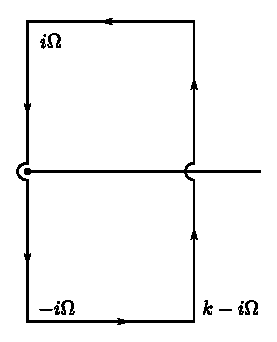
\includegraphics{vol2-figures/fig2.40.eps}}
\end{figure}

So the residue at $\mathfrak{z}=0$ is 
$$
\frac{k^2}{\pi^2 h} \left(- \frac{\pi^2}{3} - \frac{\pi^2}{3k^2} -
\frac{\pi^2 h^2}{3k^2} \right)= - \frac{k}{3 \pi} \left( \frac{k}{h} +
\frac{1}{hk} + \frac{h}{k}\right)
$$

So 
\begin{align*}
  \sum (\Res) & = - \frac{k}{3 \pi} \left(\frac{k}{h} + \frac{h}{k} +
  \frac{1}{hk}\right)+ \frac{1}{\pi} \sum^{k-1}_{\ell=1} \cot
  \frac{\pi \ell}{k} \cot \frac{\pi h \ell}{k}\\ 
  & \hspace{3cm}+ \frac{k}{\pi h}
  \sum^{h-1}_{k=1} \cot \frac{\pi r h}{h} \cot \frac{\pi h}{h}\\
  & = \frac{k}{3 \pi} \left(- \left(\frac{k}{h} + \frac{h}{k} +
  \frac{1}{hk} \right) + 12 s(h, k)+ 12 s(k, h)\right) 
\end{align*}

And\pageoriginale this is equal to 
$$
\frac{1}{2 \pi i} \int_R f(\mathfrak{z}) d \mathfrak{z}
$$
where $R$ is the rectangle. On the vertical lines the function the
same value (by periodicity) end so the integrals cancel out. Hence
$$
\frac{1}{2 \pi i} \int_R f(\mathfrak{z}) d \mathfrak{z} = \frac{1}{2
  \pi i} \left\{\int\limits^{- i \Omega + k}_{- i \Omega}-
\int\limits^{i \Omega + k}_{i \Omega} \right\}
$$

Now 
\begin{align*}
  \cot \omega & = i \frac{e^{i \omega}+ e^{- i \omega}}{e^{i \omega}-
    e^{-i \omega}}, \omega = x+ iy,\\
  & = i \frac{e^{ix-y}+e^{-ix+y}}{e^{i x-y}- e^{- ix + y}};
\end{align*}
$x$ varies from $o$ to $k$ and $y= \pm \Omega$, for this
$$
\to 
\begin{cases}
  -i, & ~\text{as}~ y= \Omega \to \infty\\
  i, & ~\text{as}~ y=- \Omega \to - \infty 
\end{cases}\qquad \text{uniformly}
$$

Therefore
\begin{align*}
  \lim\limits_{\Omega \to \infty} \frac{1}{2 \pi i} \int_R
  f(\mathfrak{z}) d\mathfrak{z} & = \frac{1}{2 \pi i} \left\{ i^3 k-
  (-i)^3 k\right\}\\
  & = \frac{2 k i^3}{2 \pi i} = - \frac{k}{\pi}
\end{align*}\pageoriginale
$$
\displaylines{\therefore \qquad \frac{k}{3 \pi} \left(- \left(
  \frac{h}{k} + \frac{k}{h} + \frac{1}{hk}\right)+ 12 s(h, k)+ 12s
  (k, h) \right) \cr
  = - \frac{k}{\pi}\cr
  \text{or} \hfill 12 s(h, k) + 12 s (k, h) = -3 + \left(\frac{k}{h} +
  \frac{h}{k} + \frac{1}{hk}\right),\hfill }
$$
which is the reciprocity formula.
